\begin{appendices}
\chapter{ }

\section{Abreviaturas}

\begin{table}[H]
\centering
\begin{tabular}{|c|p{10cm}|}
\hline 
 \textbf{ABREVIATURA} & \textbf{SIGNIFICADO} \\ 
\hline 
 AG & Algoritmo Genético \\ 
\hline 
 CdC & Ciencias de la Computación \\ 
%\hline 
% ESIME & Escuela Superior de Ingeniería Mecánica y Eléctrica\\ 
\hline 
 Facultad & Facultad de Ciencias de la UNAM \\ 
\hline 
 FES & Facultad de Estudios Superiores \\
\hline 
 ITAM & Instituto Tecnológico Autónomo de México \\ 
\hline 
 MatAp & Matemáticas Aplicadas \\ 
\hline 
 TC & Tiempo Completo \\ 
\hline 
 UNAM & Universidad Nacional Autónoma de México \\ 
\hline 
 URL & Uniform Resource Locator \\ 
\hline 
 NP & Problema que se puede resolver en un tiempo polinomial no determinístico \\ %\url{https://mathworld.wolfram.com/NP-Problem.html}
\hline 
 NP-duro & Problema tan o más difícil de resolver que un NP \\ %\url{https://mathworld.wolfram.com/NP-HardProblem.html}
\hline 
% a & b \\ 
%\hline 
\end{tabular} 
\caption[\textit{Abreviaturas}]{\textit{Abreviaturas utilizadas a lo largo de este trabajo.}}
\end{table}


%\appendix
%\chapter{Appendix Title}
%\input{chapters/appendix}
%\chapter{Resultados útiles} \label{Apend_ResultadosUtiles}
\section{Estimador máximo verosímil de $\lambda$} \label{Apend_ResultadosUtiles}

Sean $X_{1}, X_{2}, \ldots, X_{n}$ una muestra aleatoria de una población con función de densidad de probabilidad $Poisson(\lambda)$. Su función de densidad es:

$$f(x) = \mathrm{e}^{-\lambda} \dfrac{\lambda^{x}}{x!}$$

Calulemos el estimador máximo verosímil de $\lambda$:

$$\mathcal{L}(X_{1}, X_{2},\ldots, X_{n}; \lambda) = \displaystyle \prod_{i = 1}^{n} \left( \mathrm{e}^{-\lambda} \dfrac{\lambda^{x_{i}}}{x_{i}!} \right) = \mathrm{e}^{-n \lambda} \dfrac{\lambda^{\displaystyle \sum_{i = 1}^{n} x_{i}}}{\displaystyle  \prod_{i = 1}^{n} x_{i}!}$$

Sacamos ln:

$$ln \mathcal{L}(X_{1}, X_{2}, \ldots, X_{n};\lambda) = -n\lambda + \displaystyle \sum_{i = 1}^{n} x_{i} ln \lambda - ln \displaystyle  \prod_{i = 1}^{n} x_{i}!$$

Derivamos con respecto a $\lambda$:

$$\dfrac{\partial}{\partial \lambda} ln \mathcal{L}(\underline{X};\lambda) = -n + \dfrac{\displaystyle \sum_{i = 1}^{n} x_{i}}{\lambda}$$

Igualamos a cero:

$$-n + \dfrac{\displaystyle \sum_{i = 1}^{n} x_{i}}{\lambda} = 0$$

Despejamos $\lambda$:

$$\hat{\lambda} = \dfrac{\displaystyle \sum_{i = 1}^{n} x_{i}}{n} = \overline{x}$$


Derivamos otra vez:

$$\dfrac{\partial^{2}}{\partial \lambda} ln \mathcal{L}(\underline{X};\lambda)  = - \dfrac{\displaystyle \sum_{i = 1}^{n} x_{i}}{\lambda^{2}} < 0$$


Por lo tanto $\hat{\lambda} = \overline{x}$ es el estimador máximo verosímil de $\lambda$ para una distribución Poisson.


\section{Materias agrupadas} \label{materias_agrupadas}

Vemos las materias que se actualizaron o cambiaron de nombre. Las negritas son los nombres que se van a utilizar.

\begin{itemize}
\item Administración = Administración Actuarial = \textbf{Administración Actuarial del Riesgo}

\item Seminario de Inteligencia Artificial = \textbf{Recuperación y Búsqueda de Información en Textos}

\item \textbf{Seminario de Aplicaciones a las Ciencias Sociales y Administrativas} = Administración de Empresas de Software = Riesgo Tecnológico = Temas Selectos de Ingeniería de Software A

\item Probabilidad y Estadística = \textbf{Probabilidad I}

\item \textbf{Mecánica Vectorial} = Cálculo Tensorial

\item Matemáticas Avanzadas de la Física = \textbf{Funciones Especiales y Transformadas Integrales} = Análisis de Fourier I = Análisis de Fourier II = Introducción a las Funciones Recursivas y Computabilidad

\item \textbf{Mecánica Analítica} = Introducción Matemática a la Mecánica Celeste

\item \textbf{Física Computacional} = Supercómputo

\item \textbf{Teoría de Gráficas} = Teoría de las Gráficas II

\item Graficas y Juegos = \textbf{Introducción a las Matemáticas Discretas}

\item Estadística I = \textbf{Inferencia Estadística}

\item Análisis de Redes = \textbf{Teoría de Redes}

\item Bases de Datos = Formación Científica I = Sistemas Manejadores de Bases de Datos = Sistemas de Bases de Datos = Grandes Bases de Datos = Fundamentos de Bases de Datos = Almacenes y Minería de Datos = \textbf{Manejo de Datos} = Programación II

\item \textbf{Análisis Numérico} = Análisis Numérico II = Temas Selectos de Análisis Numérico

\item \textbf{Seminario sobre Enseñanza de las Matemáticas I} = Seminario de Filosofía de la Ciencia I = Didáctica de las Matemáticas

\item Estadística II = \textbf{Modelos no Paramétricos y de Regresión} = Análisis de Regresión

\item Teoría de la Computación = \textbf{Autómatas y Lenguajes Formales}

\item Matemáticas Discretas = \textbf{Estructuras Discretas}

\item Programación I = \textbf{Programación}

\item \textbf{Procesos Estocásticos I} = Procesos Estocásticos

\item \textbf{Seminario de Geometría A} = Álgebra Geométrica = Geometría Algebraica II

\item Fianzas = Matemáticas Actuariales del Seguro de Daños = \textbf{Matemáticas Actuariales para Seguro de Daños, Fianzas y Reaseguro} = Matemáticas Actuariales para Seguro de Daños = Reaseguro = Reaseguro Financiero

\item Teoría de Juegos I = \textbf{Teoría de Juegos en Economía}

\item Finanzas II = \textbf{Métodos Cuantitativos en Finanzas}

\item Seminario de Aplicaciones Actuariales I = Seminario de Matemáticas Actuariales Aplicadas = Seminario de Aplicaciones Actuariales II = \textbf{Seminario de Aplicaciones Actuariales}  = /Seminario de Aplicaciones Actuariales I/Seminario de Estadística I = Seminario de Probabilidad A = Teoría de la Medida II

\item Finanzas I = \textbf{Mercados Financieros y Valuación de Instrumentos} = Valuación de Opciones

\item Problemas Socio-Económicos de México = \textbf{Análisis del México Contemporáneo} = México: Nación Multicultural

\item Formación Científica II = \textbf{Economía} = Economía I

\item Productos Financieros Derivados I = Productos Financieros Derivados II = \textbf{Productos Financieros Derivados} 

\item Economía II = \textbf{Temas Selectos de Economía} = Econometría II 

\item Demografía I = Demografía II = \textbf{Demografía} = Demografía Avanzada

\item Introducción a Ciencias de la Computación I = Introducción a Ciencias de la Computación II = \textbf{Introducción a Ciencias de la Computación} = Estructuras de Datos = Robótica

\item Arquitectura de Computadoras = \textbf{Organización y Arquitectura de Computadoras}

\item Análisis de Algoritmos I = Análisis de Algoritmos II = \textbf{Análisis de Algoritmos}

\item \textbf{Lenguajes de Programación} = Lenguajes de Programación y sus Paradigmas = Semántica y Verificación

\item Seminario de Ciencias de la Computación A = \textbf{Seminario de Ciencias de la Computación} = Seminario de Ciencias de la Computación B = Seminario de Temas Selectos de Computación = Seminario de Aplicaciones de Cómputo = Seminario de Computación Teórica = Seminario de Aplicaciones de Cómputo II = Seminario de Sistemas para Cómputo B = Seminario de Computación Teórica II = Seminario de Sistemas para Cómputo A  = Administración de Sistemas Unix/Linux = Sistemas de Información Geográfica = Métodos Formales

\item Principios de Computación Distribuida= Computación Concurrente = \textbf{Computación Distribuida}

%\item \textbf{Animación por Computadora} (255) = \textbf{(203)}

\item Seminario de Programación = \textbf{Modelado y Programación} = Diseño y Programación Orientada a Objetos = Programación Funcional y Lógica = Programación de Dispositivos Móviles = Programación Declarativa

\item Análisis Lógico = \textbf{Lógica Computacional} = Lógica Computacional II = Lógicas no Clásicas

\item Diseño de Sistemas Digitales = \textbf{Diseño de Interfaces de Usuario} = Diseño de interfaces

\item Seminario de Inteligencia Artificial II = Reconocimiento de Patrones = \textbf{Reconocimiento de Patrones y Aprendizaje Automatizado} = Seminario de Temas Selectos de Computación II = Computación Cuántica I = Computación Cuántica II = Sistemas Expertos = Razonamiento Automatizado

\item \textbf{Seminario Filosofía de las Matemáticas} = Seminario de Filosofía de la Ciencia II = Seminario de Filosofía de la Ciencia III = Seminario de Filosofía de la Ciencia IV

\item Estadística III = \textbf{Modelos de Supervivencia y de Series de Tiempo} =  Series de Tiempo

\item \textbf{Seminario Matemáticas Aplicadas I} = Seminario de Cálculo de Formas Diferenciales

\item Seminario de Investigación de Operaciones = \textbf{Temas Selectos de Investigación de Operaciones}

\item Temas Selectos de Ingeniería de Software B = Temas Selectos de Ingeniería de Software A = Tecnologías para Desarrollos en Internet = \textbf{Ingeniería de Software II} = Patrones de Diseño de Software

\item Diseño de Experimentos = \textbf{Seminario de Estadística I}

\item \textbf{Seminario de Topología B} = Topología Diferencial II

\item \textbf{Mercadotecnia de Seguros} = Contabilidad de Seguros

\item \textbf{Graficación por Computadoras} = Visualización = Geometría Computacional = Visión Por Computadora

\item Seminario de Ciencias Computacionales = \textbf{Taller de Herramientas Computacionales} = Sistemas Dinámicos Computacionales I = Lingüística Computacional = Herramientas de Computación para las Ciencias = Algoritmos de Apareamiento de Cadenas

\item Redes Neuronales y Autómatas Celulares = \textbf{Redes Neuronales}

\item Procesos Paralelos y Distribuidos = \textbf{Algoritmos Paralelos}

\item Algoritmos Genéticos = \textbf{Cómputo Evolutivo}

\item Simulación y Control = \textbf{Control Estadístico de la Calidad}

\item Introducción a la Criptografía = \textbf{Criptografía y Seguridad}

\item \textbf{Seminario de Apoyo a la Titulación en Ciencias de la Computación} = Seminario de Apoyo a la Titulación en Ciencias de la Computación A = Seminario de Apoyo a la Titulación en Ciencias de la Computación B 

\item \textbf{Seminario de Apoyo a la Titulación en Matemáticas} = Seminario de Apoyo a la Titulación en Matemáticas A = Seminario de Apoyo a la Titulación en Matemáticas B
\end{itemize}%Fin de materias con múltiples nombres


\section{Ejemplo de asignación final} \label{Ej_AsigFinal}

Sabemos que la asignación final es el mejor elemento de la última generación. Éste elemento es la matriz que presentamos a continuación. Cabe aclarar que los datos se ordenaron con respecto a la materia (en orden alfabético) y por hora (de menor a mayor). La matriz tiene 682 grupos asignados, cada uno con materia, profesor y horario correspondiente.

\dfNmatAsigFinal

%\section{Notas} %

\begin{enumerate}
  
  \item Cuando se hacen comparaciones se toman los valores reales y se les restan los valores simulados $(Reales - \mathbb{E}[Simulados])$

  \item Para las simulaciones se utiliza la información anterior a la del semestre que se quiere simular para no tener información real dentro  de los datos para la simulación.
  
  \item Las matrices \textit{m\_grande} y de \textit{m\_grande\_total} tienen información real.
  
  \item El vector \textit{vec\_excepciones} tiene las posibles excepciones en las que las funciones que extraen información pueden caer, de esta manera se pueden generar nuevas funciones para corregir esos casos.
  
  \item La siguiente imagen es el resultado de la función \textit{imprime\_info\_idiomas} la cual muestra la información de los idiomas. Dicha función arroja un vector con los semestres que requieren modificación.

\begin{figure}[H]
\centering
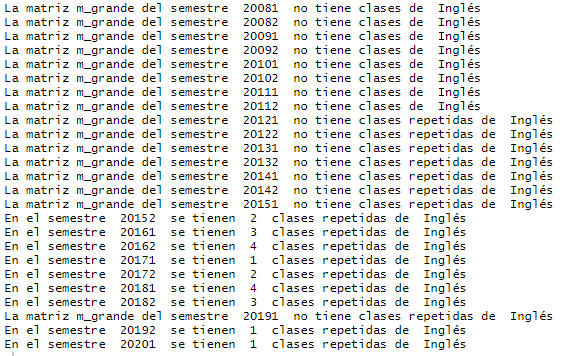
\includegraphics[scale = 0.8]{clases_de_ingles} %width=\textwidth
\caption{\textit{Resumen de clases de inglés antes de modificación}}
\end{figure}
  
Con esta información se decidió observar caso por caso los renglones que requieren modificación para la matriz \textit{m\_grande}


  \item Debido a la situación en la que estamos viviendo actualmente, ahora más que nunca es necesario tener un programa para la asignación de horarios. Que permita la realización de las asignaciones sin tener la necesidad de hacer reuniones en persona. Al proseguir con las medidas de distanciamiento social, las reuniones antiguamente hechas en persona se tendrían que hacer por medio de alguna plataforma digital. Éstas no necesariamente son las más óptimas ya que dependen de la señal de todos los participantes para que haya una comunicación de manera fluída. Debido a ésto, el programa es una buena solución.
  
  \item La información que se puede encontrar actualmente (debido a la pandemia) en las páginas web de los horarios de la Facultad no es la misma que la mostrada a lo largo del trabajo ya que ahora no se tiene información del salón, o del número de alumnos inscritos por materia, ni los lugares disponibles por grupo.
  
\begin{figure}[H]
\centering
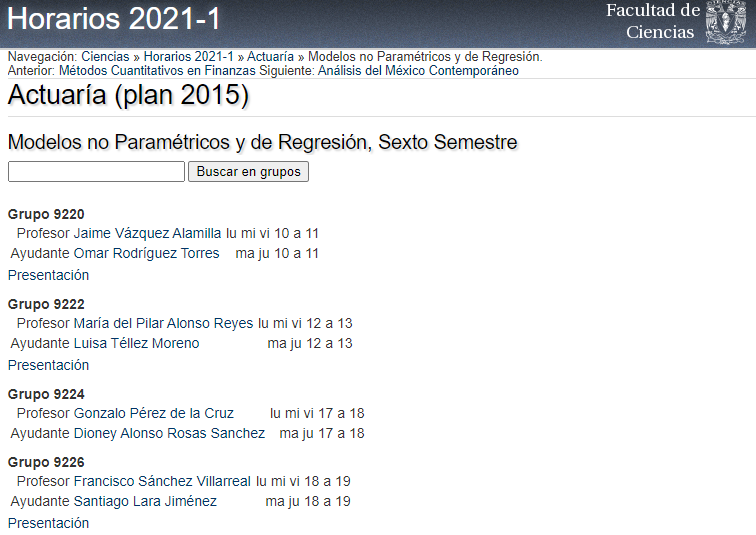
\includegraphics[scale = 0.7]{Ej_horarios_20211} %width=\textwidth
\caption{\textit{Ejemplo de horarios de semestre 2021-1}}
%\url{http://www.fciencias.unam.mx/docencia/horarios/20211/2017/1639}
\end{figure}
   
  \item La imagen \ref{img_en_ing_2} tiene título en inglés, se tienen 2 opciones: dejarlo así o buscar cómo cambiarlo.
   
  \item Arrigo dijo que posiblemente alguien se va a quejar de no tomar en cuenta la preferencia de los profesores al realizar las solicitudes.
  
  \item Cláusula 99 CCTPA: Ayuda para la impresión de la tesis.
  
  \url{https://www.personal.unam.mx/Docs/Contratos/AAPAUNAM20132015.pdf}

\begin{figure}[H]
\centering
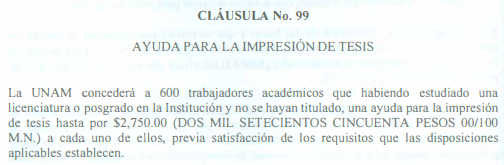
\includegraphics[scale = 1]{clausula99_CCTPA} %width=\textwidth
\caption{\textit{Cláusula 99 CCTPA: Ayuda para la impresión de la tesis}}
\end{figure}
  
  \item La frecuencia relativa en los histogramas no refleja directamente el porcentaje. Se debe multiplicar el valor del eje $Y$ por el ancho del intervalo por $100$ para obtener cifras en porcentaje. El área total de las barras sumará 1 (\ref{MargaritaJaimeRuthLizbeth}).
  
  \item Las materias que se actualizaron o cambiaron de nombre se pueden ver en el Apéndice \ref{materias_agrupadas}.
  
	\item Arrigo dijo que posiblemente alguien se va a quejar del hecho de que actualmente las inscripciones ya no se hacen con tira de materias firmada.
  
  \item How to write your PhD thesis (without going insane) \url{https://www.youtube.com/watch?v=pM6orL-bGDc&ab_channel=JamesHaytonPhD}:
  
  \begin{itemize}
    \item Definir tiempos de trabajo y tiempos de trabajo.
  
  \item Ser constante. Escribir al menos una página al día.
  
  \item Escribir más de las áreas en las que se tiene mayor conocimiento que en temas que no se conocen al 100\%.
  
  \item Si se tiene un nivel de habilidad medio y el nivel del problema/reto es alto, entonces basta que uno se concentre en el problema para poder resolverlo.
  
\begin{figure}[H]
\centering
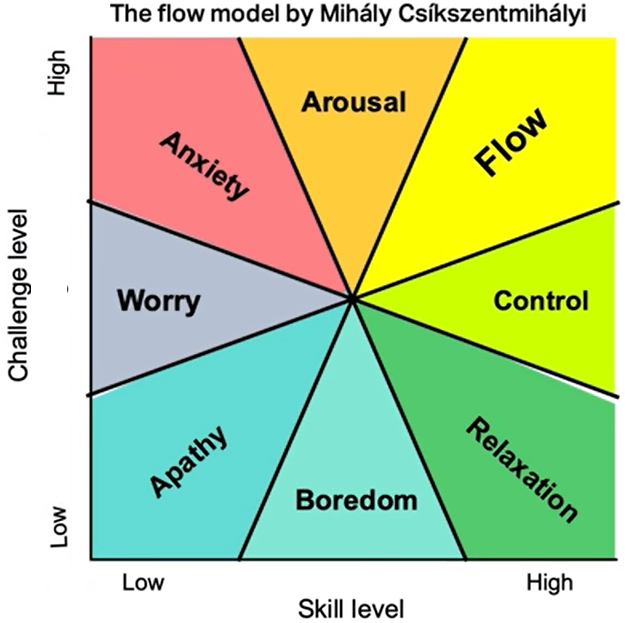
\includegraphics[scale = 0.65]{skill_vs_challenge_level} %width=\textwidth
\caption{\textit{Skill vs challenge level}}
\end{figure}  
  
  \end{itemize}
  
  \item Un programa de computadora, con que haga los mismos errores que un humano, es bueno porque su costo es menor.
    
  \item No se da 2 veces la misma materia al mismo profesor para que los alumnos tengan mayor gama de profesores para elegir.
    
  \item $X_{4}:$ Analizar presentación: Hacer varias pruebas con distintas combinaciones y elegir el mejor estilo/presentación.
  
  \item $X_{14}:$ Revisar/Investigar al respecto del problema y resolverlo.

\end{enumerate}

\end{appendices}

